\section{Tools}\label{tools}

\subsection{Code Editor}\label{codeEditor}

Blue uses the Netbeans Code Editor library for editing code. The editor
is customized depending on where you are in the application, but there
are common features shared. Some things which are available are:

\begin{itemize}
\item
  Syntax Highlighting
\item
  Code Completion (ctrl-space)
\item
  Line Numbering (enabled globally in program settings)
\item
  Popup Menu (use right-mouse click) with additional options
\end{itemize}

You can adjust colors, fonts, and other settings within Blue's Program
Options.

\subsection{BlueShare}\label{blueShare}

BlueShare

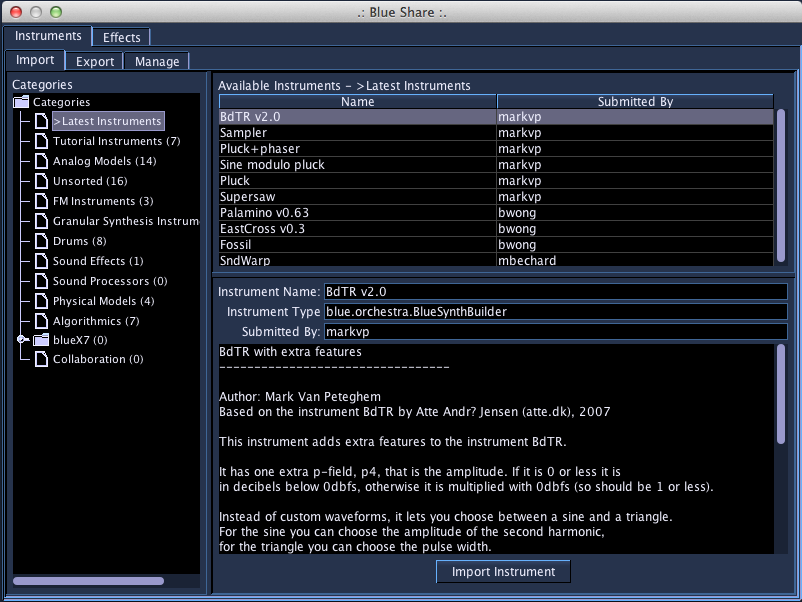
\includegraphics[width=1.00000\textwidth]{images/blueShare.png}

BlueShare is an online, in-program way to share instruments and effects
with other Blue users. BlueShare does not require a user account to
download items, but does require one for uploading. If you would like to
share an instrument or effect, please sign up for an account at
\url{http://blue.kunstmusik.com}

To use BlueShare, go to the Tools menu to open it up. Blue will contact
the server to get a list of Instrument and Effects available. From
there, you can browse categories, then select an item in the upper-right
table to get more information. Once you find something you are
interested to try, select "Import Instrument" or "Import Effect". The
instrument or effect will download to your User Instrument Library or
Effects Library in a folder called "Imported Instruments" or "Imported
Effects".

To use BlueShare, go to the Tools menu to open it up. Blue will contact
the server to get a list of Instrument and Effects available. From
there, you can browse categories, then select an item in the upper-right
table to get more information. Once you find something you are
interested to try, select "Import Instrument" or "Import Effect". The
instrument or effect will download to your User Instrument Library or
Effects Library in a folder called "Imported Instruments" or "Imported
Effects".

To upload and instrument or effect, switch to the Export tab. From there
you will see a place to enter your username and password, a listing of
instruments or effects from your libraries, a tree of categories to use
for uploading, and a description box (pre-populated with the Comments
field of your Instrument or Effect). You can then press the "Submit"
button to send it to the server.

The manage tab allows you to pull down a list of your contributed
instruments and effects. You can then remove the item from blueShare
using "Remove" button.

\subsection{Code Repository}\label{codeRepository}

Code Repository

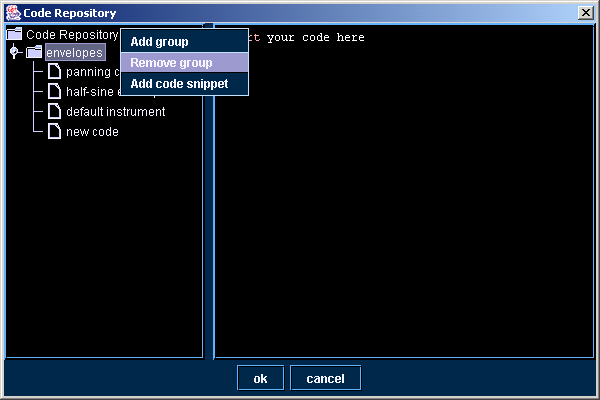
\includegraphics{images/codeRepository.png}

The Code Repository is where you edit the options that will come up from
the code popup (the popup menu that is accessible by rt-clicking on most
of the text areas in Blue).

The Code Repository features a tree to organize your code. Rt-clicking
on a folder will give you options to add a new code group, remove the
current group, or add a code snippet to the group.

If you add either a code group or a code snippet it will be created with
a default name. To edit the name, double click on the group or snippet
and the area on the tree will change into a text field to edit the name.

To edit a snippet, simply click on the snippet in the tree and on the
right a text area will appear. In that text area, edit the text that is
associated with the code snippet.

When you are done editing your code repository, the next time you
rt-click on a text area, the code popup will reflect the changes you
have made, including any new code groups and snippets you've added.

\subsection{Effects Library}\label{effectsLibrary}

The Effects Library organizes Effects used with Blue's mixer. You can
create and edit Effects, as well as organize Effects into Groups. The
layout of the tree that contains the effects will be used when building
the popup menu in the Mixer for selecting effects.

\begin{quote}
\textbf{Note}

This information will be further expanded and moved into a new section
with the manual reorganization, planned for after Blue 2.3.0.
\end{quote}

\subsection{.csoundrc Editor}\label{csoundrcEditor}

.csoundrc Editor

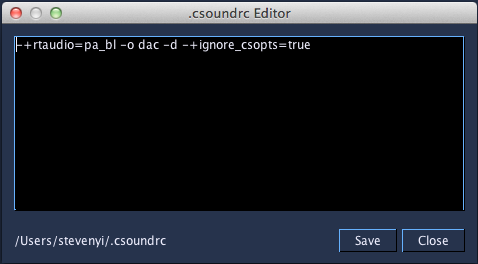
\includegraphics{images/csoundrc_editor.png}

The .csoundrc Editor tool allows for editing the system-wide .csoundrc
file. The editor is accessible from the Tools menu and launching it will
open up the file pointed to by the environment variable CSOUNDRC or
search for the file in \$HOME/.csoundrc. If neither is found, the editor
will open up with a file pointing to \$HOME/.csoundrc.

When the dialog opens, the contents (if a file is found) is shown to
edit in a simple text area. The absolute path of the file found is shown
in the bottom left hand side. Pressing the Save button will save the
contents and close the dialog, and pressing the Close button will close
the dialog without changes.

For more information about .csoundrc, please view the Csound Manual
entry for
\href{http://www.csounds.com/manual/html/CommandUnifileParFile.html}{Command
Line Parameter File (.csoundrc)}.

\subsection{Scanned Synthesis Matrix Editor}\label{scannedSynthesisMatrixEditor}

Scanned Synthesis Matrix Editor

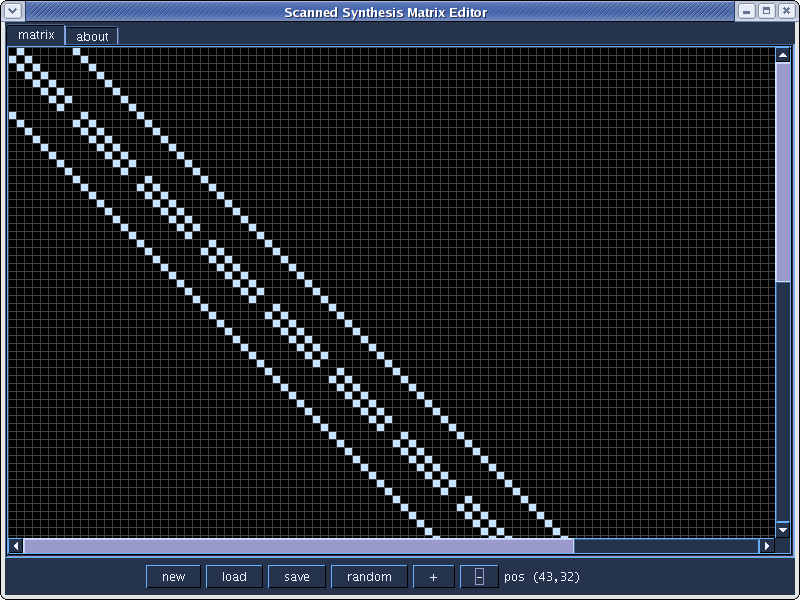
\includegraphics{images/scannedSynthesisMatrixEditor.png}

The Scanned Synthesis Matrix Editor tools allows for editing and
creating matrix files used by the Scanned Synthesis opcodes in Csound.

\begin{itemize}
\tightlist
\item
  Using "New" will ask what size matrix to create.
\item
  For editing, click anywhere on the matrix. This will either turn on or
  turn off that square, setting the connection between the masses to
  either 1 or 0.
\item
  After editing, press "Save" to save out the matrix to a file.
\item
  You can also click the "Random" button to create a randomized matrix.
\end{itemize}

\subsection{Sound Font Viewer}\label{soundFontViewer}

Sound Font Viewer

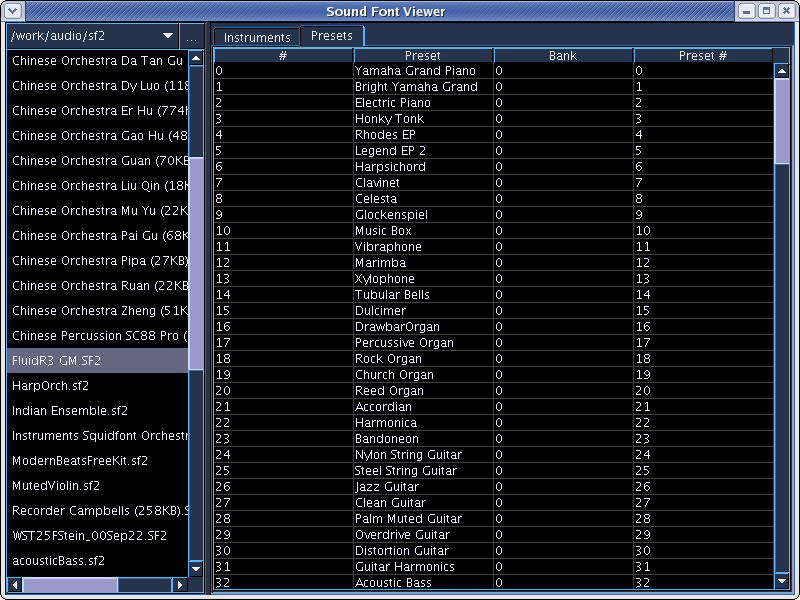
\includegraphics{images/soundFontViewer.png}

The Sound Font Viewer allows you to select SoundFonts from the file
selection panel (on the left) and get a listing of the instruments and
presets within that SoundFont.

To use, navigate using the file selection panel and double-click on a
SoundFont. After processing is complete, the tables on the right side
will be populated with a listing of instruments and presets held within
that SoundFont.

\subsection{FTable Converter}\label{ftableConverter}

FTable Converter

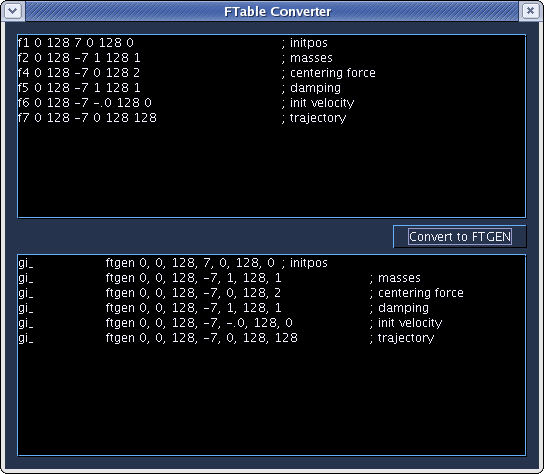
\includegraphics{images/ftableConverter.png}

The FTable Converter tool converts ftable statements into ftgen
statements. When converted, the prior ftable statement numbers are
ignored and ftgen statements are created using requested ftable number
of 0. The generated ftgen statements generate with the values of the
ftables set to "gi\_" with the expectation that the user will fill out
the rest of the name to be meaningful to them.

Conversion of ftable statements to ftgen statements is useful in
creating ftables that will be referenced by global variables instead of
hard-coded numbers.

To use, simply put your ftable statement text in the top text area and
press the "Convert to FTGEN" button to convert. For example, if you use
the following ftable statement text:

\begin{verbatim}
f1 0 128 7 0 128 0      ; initpos
f2 0 128 -7 1 128 1     ; masses
f4 0 128 -7 0 128 2     ; centering force
f5 0 128 -7 1 128 1     ; damping
f6 0 128 -7 -.0 128 0   ; init velocity
f7 0 128 -7 0 128 128   ; trajectory
\end{verbatim}

you will get the following output:

\begin{verbatim}
gi_ ftgen 0, 0, 128, 7, 0, 128, 0   ; initpos
gi_ ftgen 0, 0, 128, -7, 1, 128, 1    ; masses
gi_ ftgen 0, 0, 128, -7, 0, 128, 2    ; centering force
gi_ ftgen 0, 0, 128, -7, 1, 128, 1    ; damping
gi_ ftgen 0, 0, 128, -7, -.0, 128, 0  ; init velocity
gi_ ftgen 0, 0, 128, -7, 0, 128, 128  ; trajectory
\end{verbatim}

This work is based on the Steven Yi's FTable Converter web page utility
located \href{http://www.csounds.com/stevenyi/ftable.html}{here}.

\subsection{Python Console}\label{pythonConsole}

Python Console

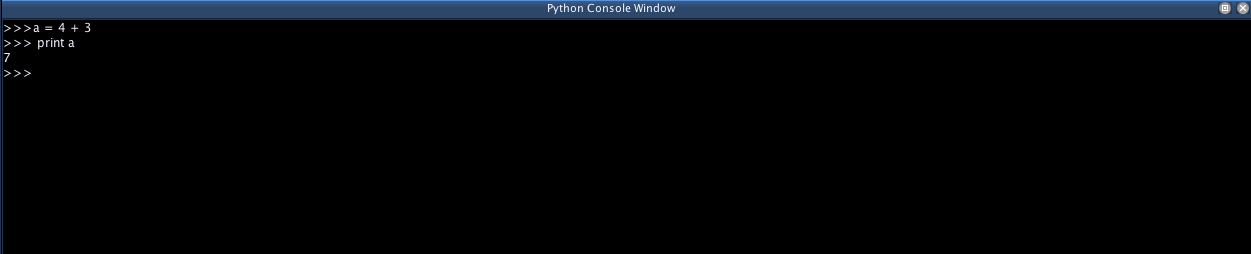
\includegraphics[width=1.00000\textwidth]{images/pythonConsole.png}

The Python Console allows you to interactively write and execute python
code using the Jython interpreter built in to Blue. Because Blue does
not clear the environment of the interpreter between runs, the console
can be useful to interactively inspect objects. Some ways you might use
the console:

\begin{itemize}
\tightlist
\item
  Use

  dir()

  to inspect objects to see what methods and members they have
\item
  Use

  help()

  to view the documentation on an object or class.
\item
  After generating a score or using the "Test" button on a PythonObject,
  you can interactively test functions you have written by calling it
  using code in the console.
\item
  Practice your python coding live.
\end{itemize}

The console works much like running python interactively in a console or
terminal. At the "\textgreater{}" prompt, you can type in some code,
then press enter to execute the code. All output from python functions
(including things like print statements in PythonObjects in the Score or
Python NoteProcessors) will output to the Python Console.

Some useful shortcuts available while in the console:

\begin{longtable}[]{@{}ll@{}}
\caption{Shortcuts for the Python Console}\tabularnewline
\toprule
Shortcuts & Description\tabularnewline
\midrule
\endfirsthead
\toprule
Shortcuts & Description\tabularnewline
\midrule
\endhead
ctrl-up/ctrl-down & cycle through previous commands used\tabularnewline
ctrl-l & clear the console (also available from the rt-click popup
menu\tabularnewline
\bottomrule
\end{longtable}
